%===============================================================================
\chapter{Controle baseado em dados}
\label{chapter:dbcd}
%===============================================================================

Neste cap�tulo ser�o apresentados conceitos b�sicos sobre projetos de controladores baseados em dados. Iniciando pela
Se��o \ref{sec:dbcd_definition}, onde ser�o abordados brevemente alguns dos mais conhecidos m�todos para projetos de
controladores baseados em dados e tamb�m os conceitos b�sicos que permeiam sua utiliza��o.

Na Se��o \ref{sec:dbcd_vrft} ser� apresentado o m�todo VRFT ({\it{Virtual reference feedback tuning}}), que
utiliza refer�ncia virtual para obten��o dos sinais necess�rios para o projeto do controlador e que ser� de grande valia
para a proposta de trabalho apresentada no Cap�tulo \ref{chapter:dbnarmax}.

Na Se��o \ref{sec:dbcd_vrft_examples} ser�o apresentados alguns exemplos de uso do m�todo VRFT e os resultados obtidos.
Ao fim, na Se��o \ref{sec:dbcd_conclusions} ser� apresentado uma breve conclus�o sobre o que foi abordado neste
cap�tulo.

%===============================================================================
%===============================================================================
\section{Defini��es}
\label{sec:dbcd_definition}
%===============================================================================

Desde meados dos anos 1990  t�m surgido na literatura uma variedade de projetos de controladores que s�o construidos
diretamente sobre os dados de entrada e sa�da coletados do sistema. Estes m�todos contrastam com os de projetos de
controladores baseados em modelos em dois aspectos principais: eles n�o s�o baseados no conhecimento do modelo do
processo e n�o t�m a inten��o de determinar livremente a fun��o de transfer�ncia do modelo. Ao inv�z disso usa-se
diretamente o montante de informa��o carregada pelos dados coletados para ajustar os par�metros de um conjunto de
modelos cuja estrutura � previamente especificada. \cite{bazanella_datadriven} 

Estes m�todos s�o conhecidos como projetos de controladores baseados em dados ou do ingl�s {\it{data-driven }} ou
{\it{data based controller design}}.

Como apresentado na se��o (\ref{sec:si_project_experiments}) estes dados podem ser obtidos de
diversas formas. Algumas vezes estas informa��es podem vir da opera��o normal da planta em malha
fechada com a presen�a de algum controlador. Situa��o esta que tem um grande apelo em plantas
industriais, onde a parada do processo, para levantamento de informa��es, � muitas vezes indesej�vel e as vezes at�
invi�vel. Se existe a possibilidade de parar a planta e aplicar sinais predeterminados, o projeto de experimentos pode
trazer muitas vantagens como foi apresentado na se��o (\ref{sec:si_project_experiments}).

O projeto de controladores baseados em dados consiste em estimar os par�metros da estrutura do controlador usando os
dados de entrada e sa�da coletados do sistema. A estimativa � feita de forma direta, ou seja, sem a necessidade de um
passo intermedi�rio para identifica��o da planta do processo. \cite{eckard_campestrini}

Existem na literatura diversos m�todos de projetos de controladores baseados em dados que otimizam algum crit�rio de
performance, com diferentes focos para diferentes crit�rios. Estes crit�rios expressam um ou uma combina��o de objetivos
fundamentais de controle: seguimento de refer�ncia, rejei��o a ru�do e uso economico da energia de controle.
Em \cite{Kammer2000} um procedimento iterativo baseado na an�lise espectral chamado de {\it{Frequency Domain Tuning}}
(FDT) foi proposto para a minimiza��o do crit�rio $H_2$ de performance para um sistema com refer�ncia zero, portanto
nenhum objetivo de seguimento de refer�ncia � almejado. O m�todo {\it{Virtual Reference Feedback Tuning}} (VRFT)
\cite{campi_leccini_savaresi2002, campi_savaresi2006} � baseado na manipula��o de vari�veis que transformam um
crit�rio $H_2$ em algo quadr�tico nos par�metros. A fun��o custo quadr�tica resultante pode ser minimizado
diretamente, sem que nenhuma itera��o seja necess�ria. Entretanto apenas o objetivo de seguimento de refer�ncia �
tratato (a n�o ser que um controlador com dois n�veis de liberdade seja usado \cite{lecchini_campi_savaresi_2dof}) e o m�nimo
global resultante desta fun��o quadr�ica coincide com o do crit�rio original somente sob condi��es ideais.
{\it{Correlation-based Tuning}} (CbT) \cite{ Karimi_cbt2003, Karimi_cbt2004} n�o sofre desta segunda limita��o, mas �
um m�todo iterativo que usa a ideia de vari�veis instrumentais para remover o efeito indesejado do ru�do enquanto
busca seu objetivo de seguimento de refer�ncia. \cite{Bazanella_h2criteria2008} 

Otimiza��o baseada em dados para um crit�rio de performance gen�rico $H_2$ foi proposto em \cite{Hjalmarsson1994}, onde
um m�todo para obter estimativas n�o polarizadas diretamente do gradiente da fun��o custo, a partir de dados do sistema
em malha fechada, foi elaborado. Este m�todo � chamado de {\it{Iterative Feedback Tuning}} (IFT). IFT � discutido a
fundo em \cite{Hjalmarsson_ift1998, Hjalmarsson2002} e extendido em \cite{Prochazka2005} para crit�rio de performances mais
gerais, que cont�m melhorias em objetivos de robustes. \cite{Bazanella_h2criteria2008} 

Na Figura (\ref{fig:vrft_db_control_loop}) � apresentado um usual sistema com realimenta��o de sa�da onde s�o
destacados os blocos do controlador, da planta e da fun��o que modifica o ru�do branco $e(t)$.

O ru�do � um processo quasi-estacion�rio, que pode ser descrito como $\nu(t)=H_0(z)e(t)$, onde
$e(t)$ � ru�do branco com vari�ncia $\sigma_e^2(t)$. Ambas fun��es de transfer�ncia, $G_0(z)$ e $H_0(z)$,
s�o racionais e causais. Assume-se que $H_0(\infty)=1$, ou seja, a resposta impulsiva do filtro
$H_0(z)$ satisfaz $h_0(0)=1$. \cite{campestrini}

\begin{figure}[htbp]
\center
% Generated with LaTeXDraw 2.0.8
% Wed Jun 20 23:11:16 BRT 2012
% \usepackage[usenames,dvipsnames]{pstricks}
% \usepackage{epsfig}
% \usepackage{pst-grad} % For gradients
% \usepackage{pst-plot} % For axes
\scalebox{1} % Change this value to rescale the drawing.
{
\begin{pspicture}(0,-1.8192188)(9.851875,1.8192188)
\pscircle[linewidth=0.04,dimen=outer](1.431875,-0.79921883){0.2}
\psframe[linewidth=0.04,dimen=outer](4.431875,-0.3992188)(2.631875,-1.1992189)
\psframe[linewidth=0.04,dimen=outer](7.231875,-0.3992188)(5.631875,-1.1992189)
\pscircle[linewidth=0.04,dimen=outer](8.431875,-0.79921883){0.2}
\psline[linewidth=0.04cm,arrowsize=0.05291667cm 2.0,arrowlength=1.4,arrowinset=0.4]{->}(0.031875,-0.79921883)(1.231875,-0.79921883)
\psline[linewidth=0.04cm,arrowsize=0.05291667cm 2.0,arrowlength=1.4,arrowinset=0.4]{->}(1.631875,-0.79921883)(2.631875,-0.79921883)
\psline[linewidth=0.04cm,arrowsize=0.05291667cm 2.0,arrowlength=1.4,arrowinset=0.4]{->}(4.431875,-0.79921883)(5.631875,-0.79921883)
\psline[linewidth=0.04cm,arrowsize=0.05291667cm 2.0,arrowlength=1.4,arrowinset=0.4]{->}(7.231875,-0.79921883)(8.231875,-0.79921883)
\psline[linewidth=0.04cm,arrowsize=0.05291667cm 2.0,arrowlength=1.4,arrowinset=0.4]{->}(8.43,0.39921868)(8.431875,-0.5992188)
\psline[linewidth=0.04cm,arrowsize=0.05291667cm 2.0,arrowlength=1.4,arrowinset=0.4]{->}(8.631875,-0.79921883)(9.831875,-0.79921883)
\psline[linewidth=0.04cm,arrowsize=0.05291667cm 2.0,arrowlength=1.4,arrowinset=0.4]{<-}(1.431875,-0.99921876)(1.431875,-1.7992188)
\psline[linewidth=0.04cm](1.431875,-1.7992188)(9.231875,-1.7992188)
\psline[linewidth=0.04cm](9.231875,-1.7992188)(9.231875,-0.79921883)
\usefont{T1}{ptm}{m}{n}
\rput(1.0698436,-0.48921886){+}
\usefont{T1}{ptm}{m}{n}
\rput(8.069845,-0.48921886){+}
\usefont{T1}{ptm}{m}{n}
\rput(8.069845,-1.0892189){+}
\usefont{T1}{ptm}{m}{n}
\rput(1.6339064,-1.0892189){-}
\usefont{T1}{ptm}{m}{n}
\rput(0.441875,-0.49921885){\small $r(t)$}
\usefont{T1}{ptm}{m}{n}
\rput(3.561875,-0.79921883){\small $C(z, \theta)$}
\usefont{T1}{ptm}{m}{n}
\rput(6.331875,-0.8192189){\small $G_0(z)$}
\usefont{T1}{ptm}{m}{n}
\rput(5.081875,-0.49921885){\small $u(t)$}
\usefont{T1}{ptm}{m}{n}
\rput(1.941875,-0.49921885){\small $\varepsilon (t)$}
\usefont{T1}{ptm}{m}{n}
\rput(8.851875,0.12078118){\small $\nu(t)$}
\usefont{T1}{ptm}{m}{n}
\rput(9.271875,-0.49921885){\small $y(t)$}
\psframe[linewidth=0.04,dimen=outer](9.231875,1.2007811)(7.631875,0.40078118)
\usefont{T1}{ptm}{m}{n}
\rput(8.411875,0.7807812){\small $H_0(z)$}
\psline[linewidth=0.04cm](8.43,1.1992186)(8.43,1.7992188)
\usefont{T1}{ptm}{m}{n}
\rput(8.871875,1.5807811){\small $e(t)$}
\end{pspicture} 
}
\caption{Representa��o de um sistema de controle em malha fechada, com ruido aditivo na sa�da. S�o apresentados tamb�m
os prncipais sinais refer�nciados.}
\label{fig:vrft_db_control_loop}
\end{figure}

A equa��o: 

\begin{equation}
T(z, \theta)=\frac{C(z,\theta)G_0(z)}{1+C(z,\theta)G_0(z)}
\label{eq:vrft_db_closed_loop}
\end{equation}

descreve a rela��o entre entrada e sa�da do sistema apresentado na Figura (\ref{fig:vrft_db_control_loop}). Desta
forma pode se escrever o sinal de sa�da do sistema como:

\begin{equation}
y(t)=T(z, \theta)r(t)
\label{eq:dbcd_def_yr}
\end{equation}


%===============================================================================
\subsection{Crit�rios de performance}
\label{sec:dbcd_performance_criteria}
%===============================================================================

Como j� foi apresentado no cap�tulo sobre identifica��o de sistemas lineares (cap�tulo
\ref{chapter:system_identification}), existe um crit�rio para elencar qual � o melhor conjunto de par�metros $\theta$
pra a classe de modelos escolhida. Para isso, foi apresentado a equa��o \eqref{eq:si_obj_etim_lsm_v} como um dos
crit�rios mais utilizados. Para projeto de controladores existem desdobramentos deste crit�rio em
fun��o dos objetivos b�sicos de controle:

\begin{itemize}
  \item Seguimento de refer�ncia,
  \item Rejei��o a ru�do e 
  \item Uso reduzido de esfor�o de controle. 
\end{itemize}

Para o objetivo de seguimento de refer�ncia, a performance por este ponto de vista pode ser avaliada pela norma:
\cite{bazanella_datadriven}

\begin{equation}
J_y(\theta)\overset{\underset{\mathrm{\Delta}}{\,}}{=}  \bar{E} \left [ y(t)-y_d(t) \right ]^2 = \bar{E}\left [
(T(z,\theta)-T_d(z))r(t) \right ]^2
\label{eq:dbcd_def_track_error}
\end{equation}

onde $y(t)$ � a sa�da medida do sistema e $y_d(t)$ � a sa�da desejada, $T_d(z)$ � o comportamento desejado para o
sistema em malha fechada.

Com base nas equa��es \eqref{eq:dbcd_def_track_error} e \eqref{eq:vrft_db_closed_loop} � poss�vel determinar o
equacionamento para o controlador ideal. Aquele que ir� fazer com que o sistema em malha fechada se comporte como o
desejado.

\begin{equation}
C_d(z)=\frac{T_d(z)}{G_0(z)(1-T_d(z))}
\label{eq:dbcd_perf_tracking_cd}
\end{equation}

Outro objetivo fundamental � minimizar o efeito do ru�do sobre a sa�da do sistema. Descreve-se a fun��o sensibilidade
$S(z, \theta)$ como:

\begin{equation}
S(z, \theta)=\frac{1}{1+C(z, \theta)G_0(z)}
\label{eq:dbcd_perf_sensitiv}
\end{equation}

A sa�da do sistema em malha fechada referente apenas ao ru�do, ou seja, sem levar em conta a parte relativa a refer�ncia
� dada por: \cite{bazanella_datadriven}

\begin{equation}
y_e(t, \theta) \overset{\underset{\mathrm{\Delta}}{\,}}{=} S(z, \theta)\nu(t)
\label{eq:dbcd_perf_ye}
\end{equation}

O crit�rio que determina a performance do sistema na rejei��o ao ru�do � dado por:

\begin{equation}
J_e(\theta) \overset{\underset{\mathrm{\Delta}}{\,}}{=} \bar{E}\left [ y_e(t) \right ]^2 = \bar{E}\left [  S(z,
\theta)\nu(t) \right ]^2
\label{eq:dbcd_perf_je}
\end{equation}

Para fazer com que $J_e(\theta)=0$ seria necess�rio que $S(z,\theta)=0 \;\;\forall z$, o que demandaria que $C(z,
\theta)G_0(z) \to \infty \;\;\forall z$, tornando desta forma imposs�vel de atingir o objetivo do crit�rio ser zero.
Relaxa-se ent�o o crit�rio de performance para:   

\begin{equation}
J_e(\theta) \overset{\underset{\mathrm{\Delta}}{\,}}{=} \bar{E}\left [ (S(z, \theta)-S_d(z,\theta))\nu(t) \right ]^2 
\label{eq:dbcd_perf_je_relax}
\end{equation}

onde $S_d(z,\theta)$ � a fun��o sensibilidade desejada para o sistema.

Assim como o controlador apresentado em \eqref{eq:dbcd_perf_tracking_cd} � o controlador �timo para o crit�rio de
performance de seguimento de refer�ncia, para o crit�rio de rejei��o ao r�ido o controlador �timo pode ser obtido. Para
minimizar a fun��o custo \eqref{eq:dbcd_perf_je} escolhe-se $T_e(z)$ como abaixo (Detalhes podem ser obtidos em
\cite{bazanella_datadriven})

\begin{equation}
T_e(z)= 1-\frac{1}{H(z)} 
\label{eq:dbcd_perf_te}
\end{equation}

Da onde obtem-se o controlador desejado para a rejei��o ao ru�do $C_e(z)$:

\begin{equation}
C_e(z)=\frac{T_e(z)}{G_0(z)(1-T_e(z))}=\frac{H(z)-1}{G_0(z)} 
\label{eq:dbcd_perf_ce}
\end{equation}

O controlador apresentado em \eqref{eq:dbcd_perf_ce} tamb�m � conhecido como controlador da minima vari�ncia.

Neste trabalho os exemplos utilizados usam-se o crit�rio de seguimento de refer�ncia, com o controlador �timo desejado
sendo representado por \eqref{eq:dbcd_perf_tracking_cd}.

%%===============================================================================
%\subsection{Iterative feedback tuning}
%\label{sec:dbcd_ift}
%%===============================================================================
%
%O m�todo IFT utiliza um algoritmo iterativo para minimizar uma fun��o custo $H_2$. O m�todo
%considera que o sistema � controlado por um controlador com dois graus de liberdade:
%
%\begin{equation}
%u(t)=C_r(z)r(t)-C_y(z)y(t)
%\label{eq:vrft_db_ift_controller}
%\end{equation}
%
%Na Figura (\ref{fig:vrft_db_ift}) � apresentado a organiza��o dos blocos dos controladores
%de \eqref{eq:vrft_db_ift_controller}, $C_r(z)$ e $C_y(z)$. O controlador pode ser
%entendido como o conjunto destes dois:\cite{Hjalmarsson_ift1998}
%
%\begin{equation}
%C(z) \equiv  \left \{ C_r(z),\, C_y(z)  \right \} 
%\nonumber
%\end{equation}
%
%\begin{figure}[htbp]
%\center
%\scalebox{1} % Change this value to rescale the drawing.
%{
%\begin{pspicture}(0,-1.68)(9.48,1.72)
%\usefont{T1}{ptm}{m}{n}
%\rput(7.691875,1.5215625){\small $\nu(t)$}
%\pscircle[linewidth=0.04,dimen=outer](4.0,0.32){0.2}
%\pscircle[linewidth=0.04,dimen=outer](8.0,0.32){0.2}
%\psframe[linewidth=0.04,dimen=outer](6.8,0.72)(5.2,-0.08)
%\psframe[linewidth=0.04,dimen=outer](2.8,0.72)(1.2,-0.08)
%\psframe[linewidth=0.04,dimen=outer](6.8,-0.88)(5.2,-1.68)
%\psline[linewidth=0.04cm,arrowsize=0.05291667cm 2.0,arrowlength=1.4,arrowinset=0.4]{->}(0.0,0.32)(1.2,0.32)
%\psline[linewidth=0.04cm,arrowsize=0.05291667cm 2.0,arrowlength=1.4,arrowinset=0.4]{->}(2.8,0.32)(3.8,0.32)
%\psline[linewidth=0.04cm,arrowsize=0.05291667cm 2.0,arrowlength=1.4,arrowinset=0.4]{->}(4.2,0.32)(5.2,0.32)
%\psline[linewidth=0.04cm,arrowsize=0.05291667cm 2.0,arrowlength=1.4,arrowinset=0.4]{->}(6.8,0.32)(7.8,0.32)
%\psline[linewidth=0.04cm,arrowsize=0.05291667cm 2.0,arrowlength=1.4,arrowinset=0.4]{->}(8.2,0.32)(9.2,0.32)
%\psline[linewidth=0.04cm,arrowsize=0.05291667cm 2.0,arrowlength=1.4,arrowinset=0.4]{<-}(6.8,-1.28)(8.0,-1.28)
%\psline[linewidth=0.04cm](8.0,-1.28)(8.0,0.12)
%\psline[linewidth=0.04cm,arrowsize=0.05291667cm 2.0,arrowlength=1.4,arrowinset=0.4]{<-}(4.0,0.12)(4.0,-1.28)
%\psline[linewidth=0.04cm](4.0,-1.28)(5.2,-1.28)
%\usefont{T1}{ptm}{m}{n}
%\rput(8.911875,0.5215625){\small $y(t)$}
%\usefont{T1}{ptm}{m}{n}
%\rput(0.481875,0.5215625){\small $r(t)$}
%\usefont{T1}{ptm}{m}{n}
%\rput(1.901875,0.3215625){\small $C_r(z)$}
%\usefont{T1}{ptm}{m}{n}
%\rput(5.951875,0.3215625){\small $G_0(z)$}
%\usefont{T1}{ptm}{m}{n}
%\rput(5.931875,-1.2784375){\small $C_y(z)$}
%\usefont{T1}{ptm}{m}{n}
%\rput(4.721875,0.7215625){\small $u(t)$}
%\psline[linewidth=0.04cm,arrowsize=0.05291667cm 2.0,arrowlength=1.4,arrowinset=0.4]{->}(8.0,1.32)(8.0,0.52)
%\usefont{T1}{ptm}{m}{n}
%\rput(4.2592187,0.1315625){-}
%\end{pspicture} 
%}
%\caption{Diagrama de bloco do sistema utilizado na identifica��o IFT.}
%\label{fig:vrft_db_ift}
%\end{figure}
%
%A fun��o custo utilizada como crit�rio no m�todo � apresentada em \eqref{eq:vrft_db_ift_j_cost}. 
%
%\begin{equation}
%J(\theta)=\frac{1}{2N}E\left [ \sum_{t=1}^{N}(L_y \tilde{y}_t(\theta))^2 +\lambda  \sum_{t=1}^{N}(L_u
%u_t(\theta))^2 \right ]
%\label{eq:vrft_db_ift_j_cost}
%\end{equation}
%
%O primeiro termo em \eqref{eq:vrft_db_ift_j_cost} � o erro entre a resposta obtida e a resposta
%desejada, balanceada por um filtro $L_y$ a segunda parte � o custo de controle balanceado pelo
%filtro $L_u$. Com $T_0(\theta)$ e $S_0(\theta)$ sendo a fun��o de transfer�ncia em malha fechada e a
%fun��o sensibilidade, respectivamente:
%
%
%\begin{equation}
%T_0(\theta)=\frac{C_r(\theta)G_0}{1+C_y(\theta)G_0}
%\nonumber
%\end{equation}
%
%\begin{equation}
%S_0(\theta)=\frac{1}{1+C_y(\theta)G_0}
%\nonumber
%\end{equation}
%
%E sendo $r$ e $\nu(t)$ independentes, \eqref{eq:vrft_db_ift_j_cost} pode ser rescrito como
%\eqref{eq:vrft_db_ift_j_cost_parts}
%
%\begin{equation}
%J(\theta)=\frac{1}{2N}\sum_{t=1}^{N}\left \{ L_y(T_d r-T_0(\theta)r) \right \}^2+\frac{1}{2} E\left [ \left \{ L_y S_0(\theta) \nu(t) \right \}^2 \right ]
%+ \lambda \frac{1}{2N}E\left [ \sum_{t=1}^{N}(L_u u_t(\theta))^2 \right ]
%\label{eq:vrft_db_ift_j_cost_parts}
%\end{equation}
%
%Onde o primeiro termo � o erro de seguimento de refer�ncia, o segundo � a contribui��o do dist�rbio
%e o terceiro � o esfor�o de controle.
%
%Para minimizar \eqref{eq:vrft_db_ift_j_cost_parts}, busca-se encontrar um ponto
%estacion�rio da equa��o, para isso calcula-se o gradiente desta equa��o e aplica-se o
%algoritmo para a converg�ncia apresentado em \eqref{eq:vrft_db_ift_algoritm}.
%\cite{hajalmson_ift_non_linear}
%
%\begin{equation}
%\theta_{i+1}=\theta_i - \gamma_i R_i^{-1}\frac{\partial J}{\partial \theta}(\theta_i)
%\label{eq:vrft_db_ift_algoritm}
%\end{equation}
%
%$R_i$ � uma matriz positiva definida, tipicamente uma estimativa da Hessiana de $J$, como por
%exemplo a aproxima��o de Gauss-Newton.
%
%Para cada itera��o $i$ em \eqref{eq:vrft_db_ift_algoritm}, o m�todo IFT necessita de dois
%experimentos, cada um de tamanho $N$. 
%

% ===============================================================================
\section{Virtual reference feedback tuning}
\label{sec:dbcd_vrft}
% ===============================================================================

% Em aplica��es pr�ticas, a descri��o matem�tica da planta n�o � dispon�vel e o sistema deve ser identificado
% baseado nas medidas obtidas deste sistema. Este assunto tem atra�do a aten��o de diversos engenheiros de
% controle desde 1940 com o pioneiro trabalho de Ziegler e Nichols (1942) com ajuste de controladores PID
% industriais. Depois do trabalho de Ziegler e Nichols diversos trabalhos surgiram, muitos em formas de
% aperfei�oamento e extens�es das t�cnicas j� apresentadas, e algumas com desenvolvimentos em novas dire��es
% (\cite{mcmillan1983tuning}, \cite{Haalman1965}). A caracter�stica principal destes m�todos � que eles podem
% ser facilmente utilizados: simples experimentos sobre a planta s�o executados e simples regras 
% s�o aplicadas sobre os dados obtidos. \cite{campi_leccini_savaresi2002}


VRFT do ingl�s {\it{Virtual reference feedback tuning}} � um m�todo direto para identifica��o de
controladores, ou seja, n�o � necess�rio o conhecimento ou identifica��o da planta para que este m�todo seja
utilizado. O m�todo se baseia na utiliza��o de apenas um conjunto de dados, n�o necessitando de experimentos
espec�ficos. O procedimento procura pelo ponto �timo do crit�rio escolhido para a identifica��o do controlador.
\cite{campi_savaresi2000}

Diferentemente de m�todos iterativos, o VRFT n�o recai sobre m�nimos locais, sempre procurando o m�nimo
global do crit�rio escolhido, sob condi��es ideais:

\begin{itemize}
  \item O sistema n�o � afetado por ru�do, ou seja, $\sigma_e^2(t)=0$.
  \item O controlador ideal $C_d(z) \in C(z, \theta)$.
  \item O controlador � parametrizado linearmente. 
\end{itemize}

O controlador a ser identificado pode ser parametrizado como abaixo:

\begin{equation}
C(z,\theta)=\beta^T(z)\theta
\label{eq:vrft_method_controller}
\end{equation}
onde $\beta(z) = \left [ \beta_1(z)\;\; \beta_2(z)\;\; \cdots \;\; \beta_n(z)\right ]^T$ � um vetor
linear de fun��es de transfer�ncias de tempo discreto e $\theta$ � o vetor de par�metros a ser estimado.

O problema de identifica��o do controlador consiste em encontrar um $\hat{\theta}$ que minimize o
crit�rio performance \eqref{eq:dbcd_def_track_error}, replicado abaixo:

\begin{equation}
J_y(\theta)\overset{\underset{\mathrm{\Delta}}{\,}}{=}  \bar{E} \left [ y(t)-y_d(t) \right ]^2 = \bar{E}\left [
(T(z,\theta)-T_d(z))r(t) \right ]^2
\nonumber
\end{equation}
que � dependente do modelo de refer�ncia escolhido. 

Apenas alguns m�todos genuinamente diretos s�o encontrados na literatura, dois destes s�o VRFT e IFT. Mesmo
estes dois m�todos pertencendo uma a mesma classe, algumas difer�n�as significativas existem e podem ser ressaltadas:
\cite{campi_savaresi2000}

\begin{itemize}
	\item {\it{IFT}} � baseado em um m�todos de gradiente decrescente e al�m disso � uma t�cnica
	iterativa. Usualmente este m�todo converge para o m�nimo local mais pr�ximo das condi��es iniciais.
	Ele requer experimentos espec�ficos sobre a planta, com entradas espec�ficas.
	\item {\it{VRFT}} � um procedimento n�o iterativo que procura pelo m�nimo global do crit�rio de
	performance \eqref{eq:dbcd_def_track_error}. Este m�todo n�o requer experimentos espec�ficos sobre
	a planta, podendo inclusive utilizar os dados do funcionamento normal do sistema.
\end{itemize}

%===============================================================================
\subsection{O m�todo}
\label{sec:dbcd_vrft_framework}
%===============================================================================

Nesta se��o ser� apresentado uma breve descri��o de como funciona o algoritmo para obten��o do controlador
utilizando o m�todo VRFT. Para maiores detalhes e discuss�es aprofundadas � indicada a leitura de
\cite{campi_savaresi2000, campi_leccini_savaresi2002, campestrini_nonminumum_phase, bazanella_datadriven}.

Suponha que o controlador $C(z, \theta)$ resulta um sistema em malha fechada cuja fun��o de
transfer�ncia � dada por $T_d(z)$. Desta forma, se $T_d(z)$ for excitado com qualquer sinal $r(t)$,
sua sa�da ser� $T_d(z)r(t)$. Uma premissa para que o sistema em malha fechada tenha a mesma
fun��o de transfer�ncia que o modelo de refer�ncia � que a sa�da dos dois sejaM a mesma para um dado
sinal $\bar{r}(t)$.

Baseado no sinal medido $y(t)$, considera-se um sinal $\bar{r}(t)$ tal que $T_d(z)\bar{r}(t)=y(t)$.
Esta refer�ncia � conhecida como {\it{virtual}} pois ela n�o existe e n�o foi utilizada para gerar o
sinal $y(t)$. A figura (\ref{fig:vrft_method_cl}) apresenta o sistema em malha fechada e os sinais
presentes.

\begin{figure}[htbp]
\center
%\scalebox{1} % Change this value to rescale the drawing.
%{
\begin{pspicture}(0,-1.4292188)(9.02,1.4692187)
\pscircle[linewidth=0.04,linestyle=dashed,dash=0.16cm 0.16cm,dimen=outer](1.4,0.97078127){0.2}
\psframe[linewidth=0.04,linestyle=dashed,dash=0.16cm 0.16cm,dimen=outer](4.8,1.3707813)(3.0,0.57078123)
\psframe[linewidth=0.04,dimen=outer](7.6,1.3707813)(6.0,0.57078123)
\psline[linewidth=0.04cm,arrowsize=0.05291667cm 2.0,arrowlength=1.4,arrowinset=0.4]{->}(0.0,0.97078127)(1.2,0.97078127)
\psline[linewidth=0.04cm,linestyle=dashed,dash=0.16cm 0.16cm,arrowsize=0.05291667cm 2.0,arrowlength=1.4,arrowinset=0.4]{->}(1.6,0.97078127)(3.0,0.97078127)
\psline[linewidth=0.04cm,arrowsize=0.05291667cm 2.0,arrowlength=1.4,arrowinset=0.4]{->}(4.8,0.97078127)(6.0,0.97078127)
\psline[linewidth=0.04cm](7.6,0.97078127)(9.0,0.97078127)
\psline[linewidth=0.04cm,linestyle=dashed,dash=0.16cm 0.16cm,arrowsize=0.05291667cm 2.0,arrowlength=1.4,arrowinset=0.4]{<-}(1.4,0.7707813)(1.4,-0.02921875)
\psline[linewidth=0.04cm,linestyle=dashed,dash=0.16cm 0.16cm](1.4,-0.02921875)(8.4,-0.02921875)
\psline[linewidth=0.04cm,linestyle=dashed,dash=0.16cm 0.16cm](8.4,-0.02921875)(8.4,0.97078127)
\usefont{T1}{ptm}{m}{n}
\rput(1.1126562,1.2807813){+}
\usefont{T1}{ptm}{m}{n}
\rput(1.6473438,0.68078125){-}
\usefont{T1}{ptm}{m}{n}
\rput(0.47,1.2707813){\small $\bar{r}(t)$}
\usefont{T1}{ptm}{m}{n}
\rput(3.99,0.97078127){\small $C(z, \theta)$}
\usefont{T1}{ptm}{m}{n}
\rput(6.76,0.9507812){\small $G_0(z)$}
\usefont{T1}{ptm}{m}{n}
\rput(5.51,1.2707813){\small $u(t)$}
\usefont{T1}{ptm}{m}{n}
\rput(2.25,1.2707813){\small $\varepsilon (t)$}
\usefont{T1}{ptm}{m}{n}
\rput(8.3,1.2707813){\small $y(t)$}
\psframe[linewidth=0.04,dimen=outer](6.0,-0.62921876)(3.8,-1.4292188)
\usefont{T1}{ptm}{m}{n}
\rput(4.91,-1.0492188){\small $T_d^{-1}(z)$}
\psline[linewidth=0.04cm](9.0,0.97078127)(9.0,-1.0292188)
\psline[linewidth=0.04cm](9.0,-1.0292188)(6.0,-1.0292188)
\psline[linewidth=0.04cm](3.8,-1.0292188)(0.0,-1.0292188)
\psline[linewidth=0.04cm](0.0,-1.0292188)(0.0,0.97078127)
\end{pspicture} 
%}
\caption{Diagrama de blocos para o m�todo VRFT. S�o destacados os sinais reais $u(t)$ e $y(t)$ al�m dos sinais virtuais
$\varepsilon (t)$ e $\bar{r}(t)$. Em pontilhado est� o controlador que quando aplicado sobre a malha, faz com que o
sistema se comporte como desejado: $T_d(z)$.}
\label{fig:vrft_method_cl}
\end{figure}

O sinal $\varepsilon(t)$ � o erro entre os sinais $y(t)$ e $\bar{r}(t)$. Sabe-se que quando a planta �
excitada com o sinal $u(t)$, o sinal $y(t)$ � obtido. Analogamente para um controlador, quando este �
excitado com o sinal $\varepsilon(t)$, o sinal $u(t)$ � obtido. A tarefa do m�todo VRFT � encontrar este
controlador, com os sinais $u(t)$ e $\varepsilon(t)$ que s�o conhecidos, a tarefa reduz-se a um problema de
identifica��o. Comumente, usa-se um pr�-filtro nos dados coletados. A ideia principal do uso deste
filtro ser� explicada posteriormente na se��o (\ref{sec:dbcd_vrft_framework_filter}). 

O algoritmo pode ser descrito pelos passos a seguir \cite{campi_savaresi2000}:

\begin{enumerate}
	\item Filtram-se os sinais de entrada e sa�da com algum filtro $L(z)$:

\begin{equation}
y_L (t)=L(z)y(t), \;\;\; u_L (t)=L(z)u(t) 
\label{eq:vrft_method_algorithm_filter_io}
\end{equation}

\begin{equation}
\varepsilon_L (t)=L(z)\varepsilon (t)=\bar{r}_L (t)-y_L (t) 
\nonumber
\end{equation}


\item Encontra-se um sinal de refer�ncia $\bar{r}_L (t)$ no qual a sa�da do modelo de refer�ncia
$T_d(z)$ seja exatamente $y_L (t)$ quando alimentado pelo sinal:

\begin{equation}
y_L (t)=T_d(z) \bar{r}_L (t)
\label{eq:vrft_method_algorithm_ref}
\end{equation}

\item Seleciona-se o vetor de par�metros do controlador $\hat{\theta}$ que minimize o crit�rio:

\begin{equation}
J_{VR}^N(\theta)=\frac{1}{N}\sum_{t=1}^{N}(u_L(t)-\varphi_L^T(t)\theta)^2
\label{eq:vrft_method_algorithm_criter}
\end{equation}

\begin{equation}
\varphi_L(t)=\beta(z)\varepsilon_L(t)
\nonumber
\end{equation}

Desde que \eqref{eq:vrft_method_algorithm_criter} seja quadr�tica em $\theta$ o vetor de par�metros
$\hat{\theta}$ que minimiza esta fun��o custo pode ser calculado por:

\begin{equation}
\hat{\theta}= \left [ \sum_{t=1}^{N}\varphi_L(t) \varphi_L(t)^T\right ]^{-1}
\sum_{t=1}^{N}\varphi_L(t) u_L(t)
\label{eq:vrft_method_algorithm_result}
\end{equation}

\end{enumerate}

Com o int�ito de exemplificar, na Figura (\ref{fig:vrft_cost_functions}) � apresentado uma curva da fun��o custo
$J_y(\theta)$ de um sistema hipot�tico, e a fun��o custo proposta pelo m�todo VRFT $J_{VR}(\theta)$, a qual � quadr�tica em $\theta$.
Ao tentar encontrar o ponto de m�nimo da curva $J_y(\theta)$ pode-se recair em algum m�nimo local, o que n�o acontece 
para a curva  $J_{VR}(\theta)$.

\begin{figure}[htbp]
\center
% Generated with LaTeXDraw 2.0.8
% Mon Jul 02 22:05:15 BRT 2012
% \usepackage[usenames,dvipsnames]{pstricks}
% \usepackage{epsfig}
% \usepackage{pst-grad} % For gradients
% \usepackage{pst-plot} % For axes
\scalebox{0.75} % Change this value to rescale the drawing.
{
\begin{pspicture}(0,-4.62)(11.799063,4.62)
\psbezier[linewidth=0.04](0.9,3.3)(2.1,3.2)(2.0225368,2.3742967)(2.1565964,1.5166456)(2.290656,0.6589943)(2.616248,-1.3127834)(3.008854,-0.5402044)(3.4014597,0.23237456)(3.6584003,0.8693678)(3.811938,0.20167358)(3.9654756,-0.4660206)(4.5199084,-3.4794219)(5.1017394,-3.533306)(5.68357,-3.5871902)(8.0,1.8)(9.5,3.2)
\psbezier[linewidth=0.04,linestyle=dashed,dash=0.16cm 0.16cm](0.4,2.2)(2.2,-2.6)(3.960841,-3.4989967)(5.12,-3.54)(6.279159,-3.5810034)(9.3,-1.9)(10.6,1.9)
\psline[linewidth=0.04cm,arrowsize=0.05291667cm 4.0,arrowlength=1.4,arrowinset=0.4]{<-}(1.1,4.6)(1.2,-4.6)
\psline[linewidth=0.04cm,arrowsize=0.05291667cm 4.0,arrowlength=1.4,arrowinset=0.4]{->}(0.0,-3.9)(11.3,-3.9)
\psline[linewidth=0.04cm,linestyle=dotted,dotsep=0.16cm](5.1,-4.0)(5.0,3.1)
\usefont{T1}{ppl}{m}{n}
\rput(5.114531,-4.19){$\theta^*$}
\usefont{T1}{ppl}{m}{n}
\rput(11.014531,-4.19){$\theta$}
\usefont{T1}{ppl}{m}{n}
\rput(0.5545313,4.01){$J(\theta)$}
\usefont{T1}{ppl}{m}{n}
\rput(2.5545313,2.71){$J_y$}
\usefont{T1}{ppl}{m}{n}
\rput(3.2145312,-1.79){$J_{VR}$}
\end{pspicture} 
}
\caption{Gr�fico da fun��o custo de algum sistema hipot�tico e a respectiva fun��o custo proposta plo m�todo VRFT que �
mais simples de encontrar o ponto de m�nimo pois � quadr�tica em $\theta$, n�o recaindo em m�nimos locais. O valor
$\theta^*$ � o ponto de m�nimo de ambas as fun��es custo, logo, minimizando a fun��o custo $J_{VR}(\theta)$ � o
equivalente a minimizar $J_y(\theta)$ sob condi��es ideais.}
\label{fig:vrft_cost_functions}
\end{figure}

%===============================================================================
\subsection{Utiliza��o do Filtro $L(z)$}
\label{sec:dbcd_vrft_framework_filter}
%===============================================================================

Considerando a fun��o custo $J_{y}(\theta)$ apresentada em \eqref{eq:dbcd_def_track_error} e o
crit�rio do m�todo de refer�ncia virtual $J_{VR}(\theta)$ apresentado em \eqref{eq:vrft_method_algorithm_criter} serem
diferentes fora de situa��es ideais. A escolha correta do filtro $L(z)$ propicia que estas duas equa��es tenham m�nimos
muito pr�ximos \cite{campi_leccini_savaresi2002}.

A utiliza��o do filtro � de grande import�ncia em situa��es onde a escolha do modelo $C(z,\theta)$ n�o consegue
representar a totalidade do controlador �timo ($C_d(z)$) que quando aplicado em conjunto com a planta proporciona a
exata resposta desejada pela escolha de $T_d(z)$, ou seja:

\begin{equation}
C_d(z) \notin C(z, \theta)
\nonumber
\end{equation}

Aplicando o teorema de Perseval  para a fun��o custo de seguimento de refer�ncia:

\begin{equation}
J_y(\theta)=\bar{E}\left [ (T(z,\theta)-T_d(z))r(t) \right ]^2
\nonumber
\end{equation}
e usando as rela��es de malha fechada:

\begin{equation}
T_d(z)=\frac{C_d(z)G_0(z)}{1+C_d(z)G_0(z)}\;\;\;\; T(z, \theta)=\frac{C(z, \theta)G_0(z)}{1+C(z, \theta)G_0(z)}
\nonumber
\end{equation}

Resultam na seguinte express�o no dominio da frequ�ncia para a fun��o custo:

\begin{equation}
J_y(\theta)=\frac{1}{2\pi}\int_{-\pi}^{\pi}\left | \frac{G_0(e^{j\omega})C(e^{j\omega},
\theta)}{1+G_0(e^{j\omega})C(e^{j\omega},\theta)}-\frac{G_0(e^{j\omega})C_d(e^{j\omega})}{1+G_0(e^{j\omega})C_d(e^{j\omega})} \right |^2 \Phi_r(e^{j\omega})d\omega
\nonumber
\end{equation}

Desenvolvendo esta express�o, pode-se descreve-la mais compactamente como:

\begin{eqnarray}\nonumber
J_y(\theta)&=&\frac{1}{2\pi}\int_{-\pi}^{\pi}\left | G_0(e^{j\omega}) \right |^2 \left | S(e^{j\omega},\theta) \right |^2\left | S_d(e^{j\omega}) \right |^2 \\
&&  \times \left | C(e^{j\omega},\theta)-C_d(e^{j\omega}) \right |^2 \Phi_r(e^{j\omega})d\omega
\label{eq:dbcd_vrft_jy_cost}
\end{eqnarray}

Adiciona-se o filtro $L(z)$ � fun��o custo do VRFT, $J_{VR}(\theta)$:

\begin{equation}
J_{VR}(\theta)=\bar{E}\left [ L(z)(u(t)-C(z,\theta)\bar{\varepsilon}(t)) \right ]^2
\nonumber
\end{equation}
e usando as rela��es:

\begin{equation}
1-T_d(e^{j\omega})=S_d(e^{j\omega})
\nonumber
\end{equation}
e

\begin{equation}
\frac{T_d(e^{j\omega})}{G_0(e^{j\omega})}=C_d(e^{j\omega})S_d(e^{j\omega})
\nonumber
\end{equation}
pode-se ent�o reescrever a fun��o custo do VRFT como :


\begin{eqnarray}\nonumber
J_{VR}(\theta)&=&\frac{1}{2\pi}\int_{-\pi}^{\pi}\left | L(e^{j\omega}) \right |^2 \frac{\left | G_0(e^{j\omega}) \right
|^2 \left | S_d(e^{j\omega}) \right |^2}{\left | T_d(e^{j\omega}) \right |^2}\\ 
 && \times \left | C_d(e^{j\omega})- C(e^{j\omega},\theta) \right |^2 \Phi_u(e^{j\omega})d\omega  
\label{eq:dbcd_vrft_jvr_cost}
\end{eqnarray}

Comparando agora \eqref{eq:dbcd_vrft_jy_cost} e \eqref{eq:dbcd_vrft_jvr_cost}, observa-se que quando $C_d(z) \in
C(z,\theta)$ as duas fun��es custo s�o iguais, possuindo tamb�m o mesmo m�nimo. Quando $C_d(z) \notin C(z,\theta)$
nenhum dos crit�rios desaparece e o ponto de m�nimo depende de v�rios fatores dentro da integral. Se os fatores dentro dos dois
integrandos s�o diferentes, n�o existe motivos para esperar que os dois custos dejam o mesmo.
\cite{bazanella_datadriven}

Existe entretanto o parametro livre que foi incluido � fun��o custo do VRFT que pode ser escolhido a fim de aproximar
estes dois integrandos: o filtro $L(z)$. Para fazer com que $J_{VR}(\theta)=J_y(\theta)$, � suficiente escolher
$L(e^{j\omega})$ como:

\begin{equation}
\left | L(e^{j\omega}) \right |^2=\left | T_d(e^{j\omega}) \right |^2\left | S(e^{j\omega},\theta) \right
|^2\frac{\Phi_r(e^{j\omega})}{\Phi_u(e^{j\omega})}, \;\;\;\; \forall\omega \in \left [ -\pi; \pi \right ]
\label{eq:dbcd_vrft_filter_l}
\end{equation}
onde $\Phi_r(e^{j\omega})$ representa o espectro do sinal real da refer�ncia $r(t)$ e $\Phi_u(e^{j\omega})$ representa o
espectro do sinal aplicado sobre o sistema, medido durante o experimento do VRFT.

O c�lculo do filtro apresentado em \eqref{eq:dbcd_vrft_filter_l} requer do conhecimento da fun��o $S(z,\theta)$, que
algumas vezes pode n�o ser conhecida. Ent�o a implementa��o deste filtro ir� recair em alguma aproxima��o desta fun��o
de transfer�ncia. Quanto melhor for a aproxima��o, mais pr�ximos ser�o os m�nimos das fun��es custo $J_y(\theta)$ e
$J_{VR}(\theta)$. \cite{bazanella_datadriven}

Entretanto esta n�o � a �nica escolha sens�vel para a aproxima��o de $S(z,\theta)$, VRFT usa invariavelmente o seguinte:

\begin{equation}
\left | S(e^{j\omega},\theta) \right |^2\approx \left | S_d(e^{j\omega}) \right |^2=\left | 1-T_d(e^{j\omega}) \right
|^2
\label{eq:dbcd_vrft_sensible_s}
\end{equation}
o que aparenta ser uma aproxima��o razoavel, uma vez que � esperado que as duas fun��es sensibilidades em
\eqref{eq:dbcd_vrft_sensible_s} sejam pr�ximas ao redor do ponto de m�nimo. Usando esta aproxima��o, a fun��o de
transfer�ncia do filtro pode ser obtida por:

\begin{equation}
\left | L(e^{j\omega}) \right |^2=\left | T_d(e^{j\omega}) \right |^2\left | 1-T_d(e^{j\omega},\theta) \right
|^2\frac{\Phi_r(e^{j\omega})}{\Phi_u(e^{j\omega})}, \;\;\;\; \forall\omega \in \left [ -\pi; \pi \right ]
\label{eq:dbcd_vrft_filter_l_vrft}
\end{equation}

Para o caso onde $C_d \in C(z, \theta)$ a escolha de $L(z)$ n�o afeta o resultado, usualmente
escolhe-se ent�o $L(z)=1$.\cite{campi_leccini_savaresi2002}

Com o fltro $L(z)$ calculado como em \eqref{eq:dbcd_vrft_filter_l_vrft}, o valor assint�tico de $\theta$ pode ser
escrito como:

\begin{equation}
\theta_*=\bar{E}\left [ \varphi_L(t)\varphi_L(t)^T  \right ]^{-1}\bar{E}\left [ \varphi_L(t)u_L(t)  \right ]
\label{eq:dbcd_vrft_filter_estim}
\end{equation}
onde $\varphi_L(t)=L(z)\varphi(t)$ e $u_L(t)=L(z)u(t)$. O c�lculo real para obter os par�metros da estimativa � dado
por:

\begin{equation}
\theta=\left [ \sum_{t=1}^{N}\varphi_L(t)\varphi_L^T(t) \right ]^{-1} \sum_{t=1}^{N}\varphi_L(t)u_L(t)
\label{eq:dbcd_vrft_filter_estim_N}
\end{equation}
e na aus�ncia de ru�do, $\theta$ � igual ao valor de $\theta_*$ apresentado em \eqref{eq:dbcd_vrft_filter_estim}.

Na figura \ref{fig:vrft_cost_functions_L} um exemplo hipot�tico, onde o valor de $\theta$ que minimiza $J_{VR}(\theta)$ se
aproxima do valor de m�nimo de $J_y(\theta)$ com a utiliza��o do filtro $L(z)$. Tamb�m observa-se que a curva de
$J_{VR}(\theta)$ quando o filtro � aplicado apresenta uma redu��o na sua concavidade, fazendo com que o valor de m�nimo
na curva encontrado pelo algoritmo seja menos preciso, aumentando o a vari�ncia das estimativas, enquanto reduz o erro
de polariza��o.

\begin{figure}[htbp]
\center
% Generated with LaTeXDraw 2.0.8
% Tue Jul 03 00:08:46 BRT 2012
% \usepackage[usenames,dvipsnames]{pstricks}
% \usepackage{epsfig}
% \usepackage{pst-grad} % For gradients
% \usepackage{pst-plot} % For axes
\scalebox{0.75} % Change this value to rescale the drawing.
{
\begin{pspicture}(0,-3.97)(11.489062,3.97)
\psbezier[linewidth=0.04,linestyle=dashed,dash=0.16cm 0.16cm](0.59,-0.85)(1.39,-1.95)(3.950841,-2.6489966)(5.11,-2.69)(6.269159,-2.7310033)(8.69,-2.05)(9.69,-0.95)
\psline[linewidth=0.04cm,arrowsize=0.05291667cm 4.0,arrowlength=1.4,arrowinset=0.4]{<-}(1.39,3.95)(1.39,-3.95)
\psline[linewidth=0.04cm,arrowsize=0.05291667cm 4.0,arrowlength=1.4,arrowinset=0.4]{->}(0.59,-3.25)(11.09,-3.25)
\usefont{T1}{ppl}{m}{n}
\rput(10.704532,-3.54){$\theta$}
\usefont{T1}{ppl}{m}{n}
\rput(0.88453126,3.36){$J(\theta)$}
\usefont{T1}{ppl}{m}{n}
\rput(1.9445312,-0.04){$J_y$}
\usefont{T1}{ppl}{m}{n}
\rput(4.804531,1.16){$J_{VR}$}
\psbezier[linewidth=0.04](0.79,1.15)(0.79,0.35)(2.8950949,-2.049184)(3.89,-2.15)(4.884905,-2.2508159)(4.788093,-1.547449)(5.59,-0.95)(6.3919067,-0.35255104)(6.676079,-1.3078374)(7.19,-0.45)(7.7039213,0.40783736)(7.61,0.85)(8.01,1.71)(8.41,2.57)(9.09,2.89)(9.59,3.05)
\psbezier[linewidth=0.04,linestyle=dotted,dotsep=0.16cm](3.69,1.55)(4.49,0.45)(5.950841,-1.8489966)(7.11,-1.89)(8.269159,-1.9310033)(10.09,0.75)(10.99,1.85)
\usefont{T1}{ppl}{m}{n}
\rput(7.8545313,-2.54){$J_{VR}^L$}
\psdots[dotsize=0.24,dotstyle=asterisk](5.29,-2.71)
\psdots[dotsize=0.24,dotstyle=asterisk](7.15,-1.91)
\psdots[dotsize=0.24,dotstyle=asterisk](4.05,-2.17)
\end{pspicture} 
}
\caption{Exemplo hipot�tico de fun��es custo na sitau��o onde o controlador ideal n�o consegue ser representado pelo
modelo. Situa��o esta que o uso do filtro $L(z)$ agrega valor reduzindo o erro de polariza��o da estimativa -
Observa-se a aproxima��o do valor de m�nimo das fun��es custo pelo uso do filtro ($J(\theta)_{VR}^L$).}
\label{fig:vrft_cost_functions_L}
\end{figure}


%===============================================================================
\subsection{Dados corrompidos por ru�do}
\label{sec:dbcd_vrft_framework_noise}
%===============================================================================

Nesta se��o ser� apresentado brevemente o comportamento do m�todo quando o sinal $y(t)$ �
corrompido por um ru�do aditivo como:

\begin{equation}
\tilde{y}(t)=G_0(z)u(t) + \nu(t)
\label{eq:vrft_framework_noise_y}
\end{equation}

Assume-se que o sinal $u(t)$ e $\nu(t)$ sejam descorrelacionados e tamb�m que os dados s�o coletados
com a planta trabalhando em la�o aberto \cite{campi_leccini_savaresi2002}. A ideia estendida
de dados coletados com a planta em la�o fechado, podem ser encontradados em \cite{lecchini}.

Ao aplicar o algoritmo descrito na se��o (\ref{sec:dbcd_vrft_framework}) com dados sujeitos a ru�dos, o
resultado obtido possui erro de polariza��o. Isso pode ser compreendido analisando a express�o do crit�rio
$J_{VR}(\theta)$ quando utiliza-se o sinal $\tilde{y}(t)$:

\begin{eqnarray}\nonumber
J_{VR}(\theta)&=&\frac{1}{2\pi} \int_{-\pi}^{\pi} \left | G_0(e^{j\omega}) \right |^2 \left |
 C(e^{j\omega},\theta)-C_d(e^{j\omega}) \right |^2 \left | 1-T_d(e^{j\omega}) \right |^2 \frac{\left | L(e^{j\omega})
 \right |^2}{\left | T_d(e^{j\omega}) \right |^2}  \Phi_u(e^{j\omega}) \\
 && + \frac{\left | C(e^{j\omega},\theta) \right  |^2}{\left | G_0(e^{j\omega}) \right |^2 \left | C_d(e^{j\omega})
 \right |^2}\left | L(e^{j\omega}) \right |^2\Phi _d \; d\omega
\label{eq:vrft_framework_noise_vr}
\end{eqnarray}
onde $\Phi_d$ � a densidade do espectro do ru�do.

Para que haja rejei��o a este rudo no m�todo, em \cite{campi_leccini_savaresi2002} foi sugerido a
adi��o da vari�vel instrumental $\zeta(t)$. Em \eqref{eq:vrft_framework_noise_iv} apresenta-se o
regressor deste instrumento:

\begin{equation}
\tilde{\varphi }_L(t)=\beta(z)L(z)\left ( T_d(z)^{-1}-1 \right )\tilde{y}(t)
\label{eq:vrft_framework_noise_iv}
\end{equation}

Os par�metros do controlador podem ent�o ser calculados como em:

\begin{equation}
\theta_{N}^{IV}=\left [ \sum_{t=1}^{N}\zeta(t) \tilde{\varphi}_L(t)^T \right ]^{-1}\left [ 
\sum_{t=1}^{N}\zeta(t)u_L(t) \right ]
\label{eq:vrft_framework_noise_theta_iv}
\end{equation}

S�o propostas duas alternativas para a escolha da vari�vel instrumental. A primeira garante
assintoticamente que $\theta_N^{IV}= \theta_0$, entretanto um experimento adicional �
requisitado. O segundo n�o garante, rigorosamente, $\theta_N^{IV}= \theta_0$ mas o erro
esperado � pequeno, al�m disso um segundo experimento n�o � necess�rio. \cite{campi_leccini_savaresi2002}

\begin{itemize}
	\item {\it{Experimento Repetido:}} Executa-se um segundo experimento com a mesma entrada $u(t)$,
	adquirindo-se a sa�da $\tilde{y}(t)'$. Como o ru�do entre um experimento e outro � independente,
	$\tilde{y}(t)$ e $\tilde{y}(t)'$ ser�o diferentes. Obt�m-se ent�o a vari�vel instrumental:
	
	\begin{equation}
	\zeta(y)=\beta(z)L(z)\left ( T_d(z)^{-1}-1 \right )\tilde{y}(t)'
	\nonumber
	\end{equation}
	
	\item {\it{Identifica��o da planta:}} Identifica-se a planta $G_0(z)$ com uma famil�a de modelos como $G(z,\theta_G)$ a
	partir do conjunto de dados $\left \{ u(t), \; \tilde{y}(t) \right \}_{t=1,..., N}$ e ent�o gera-se o sinal simulado
	$\hat{y}=G(z,\theta_G)u(t)$, obtendo a vari�vel instrumental como:

	\begin{equation}
	\zeta(y)=\beta(z)L(z)\left ( T_d(z)^{-1}-1 \right )\hat{y}(t)
	\nonumber
	\end{equation}
	
	Devido as incertezas na estimativa de $G(z,\theta_G)$, este segundo m�todo n�o garante que a
	estimativa tenda assintoticamente a $\theta_0$.
\end{itemize}

%===============================================================================
\subsection{Exemplos ilustrativos}
\label{sec:dbcd_vrft_examples}
%===============================================================================

Nesta se��o ser�o apresentados alguns exemplos ilustrativos da utiliza��o do m�todo do VFRT. Ser�o utilizados sistemas
lineares modelados pelas classes de modelos ARX e BJ quando o controlador $C(z, \theta)$ faz parte da classe de
controladores que representa completamente o controlador ideal e tamb�m um caso onde o controlador ideal $C_d(z)$ n�o
consegue ser presentado pela classe de controlador escolhida.

Nas identifica��es apresentadas a seguir ser� sempre utilizado um sinal PRBS de ordem 7.

%===============================================================================
\subsubsection{Controlador PI - sistema Box-Jenkins}
\label{sec:dbcd_vrft_examples_pi_bj}
%===============================================================================

Considere o sistema real definido como:

\begin{equation}
G_{ 0 }(z)=\frac { 0.5 }{ z-0.85 } ,\quad \quad \quad H_{ 0 }(z)=\frac { z }{
z-0.4 } 
\nonumber
\end{equation}

Este sistema pode ser compreendido como um sistema {\it{Box-Jenkins}} (BJ)
(Tabela (\ref{table:si_modeling_models})). Deseja-se que o sistema em malha
fechada comporte-se o mais pr�ximo poss�vel de:

\begin{equation}
T_d(z)=\frac { 0.4 }{ z-0.6 }
\label{eq:vrft_methos_ex_bj_M}
\end{equation}

Tem-se assim que o controlador ideal pode ser definido por:

\begin{equation}
C_d(z)=\frac{T_d(z)}{G_0(z)(1-T_d(z))} = \frac { 0.8(z - 0.85) }{ z-1 }
\label{eq:vrft_methos_ex_bj_cd}
\end{equation}

Observa-se que este controlador pode ser representado como um controlador {\it{PI}} como em: 

\begin{equation}
C(z, \theta)=\frac { \theta_1 z +\theta_2}{ z-1 }
\label{eq:vrft_methos_ex_bj_c}
\end{equation}

Escolheu-se \eqref{eq:vrft_methos_ex_bj_c} como sendo a classe de modelos a ser utilizada para a identifica��o do
controlador.

Utilizando o m�todo do VRFT para identifica��o do controlador quando este est� submetido a um ru�do $\sigma_e^2=0.005$
obt�m-se a estimativas dos par�metro s $\theta_1$ e $\theta_2$ apresentados na Figura (\ref{fig:vrft_bj_M10_var005})
com um resultado de 100 simula��es com $N=2540$ cada.

\begin{figure}[htbp]
	\center
	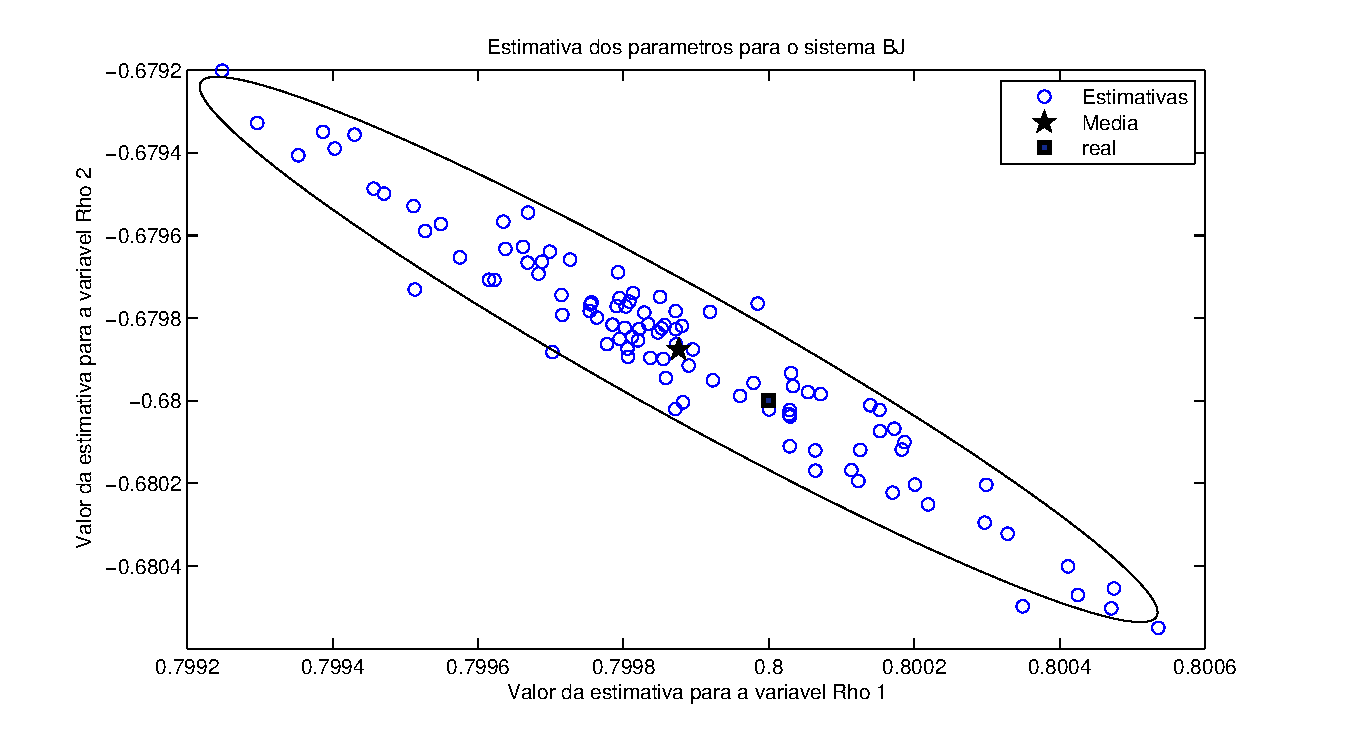
\includegraphics[width=0.95\columnwidth]{figures/vrft_bj_M10_var005.eps}
	\caption{Resultado das 100 estimativas de Monte Carlo dos par�metros $\theta_1$ e $\theta_2$ para o controlador
	apresentado em \eqref{eq:vrft_methos_ex_bj_c}. Adicionado a simula��o um ru�do aditivo de vari�ncia $\sigma_e^2=0.005$}
	\label{fig:vrft_bj_M10_var005}
\end{figure}

Os par�metros reais esperados para o controlador (equa��o \eqref{eq:vrft_methos_ex_bj_cd}) e a m�dia de todas
as estimativas $\hat{\theta}_N$ (valor representado por uma estrela na Figura (\ref{fig:vrft_bj_M10_var005})) n�o s�o os
mesmos. Em uma situa��o onde o erro de polariza��o das estimativas n�o existe, o aumento de N (n�mero de
amostras) implica que esta diferen�a diminui, tendendo a zero. Em um cen�rio onde h� erro de polariza��o, se 
aumentarmos a vari�ncia do ru�do do sistema, ser� observado um aumento desta diferen�a.

\begin{equation}
\lim_{N \rightarrow \infty }\hat{\theta}_N = \theta_0
\nonumber
\end{equation}

Na figura (\ref{fig:vrft_bj_M10_var02})  � apresentado o resultado para a estimativa de $\theta$ quando a vari�ncia do 
ru�do � quadruplicada ($\sigma_e^2=0.02$). Observa-se ent�o que o erro de polariza��o existe na estimativa. Como
descrito em \cite{campi_leccini_savaresi2002} quando o m�todo do VRFT � utilizado com ru�do nas amostras, a estimativa
� inevitavelmente polarizada. Na se��o (\ref{sec:dbcd_vrft_framework_noise}) foi sugerido o uso de vari�veis
instrumentais par para que este erro de polariza��o seja minimizado. Utilizou-se ent�o este m�todo e para um ru�do com
a mesma vari�ncia ($\sigma_e ^2=0.02$), o resultado �btido � o apresentado na Figura (\ref{fig:vrft_bj_M10_var02_iv}).

\begin{figure}[htbp] 
	\center 
	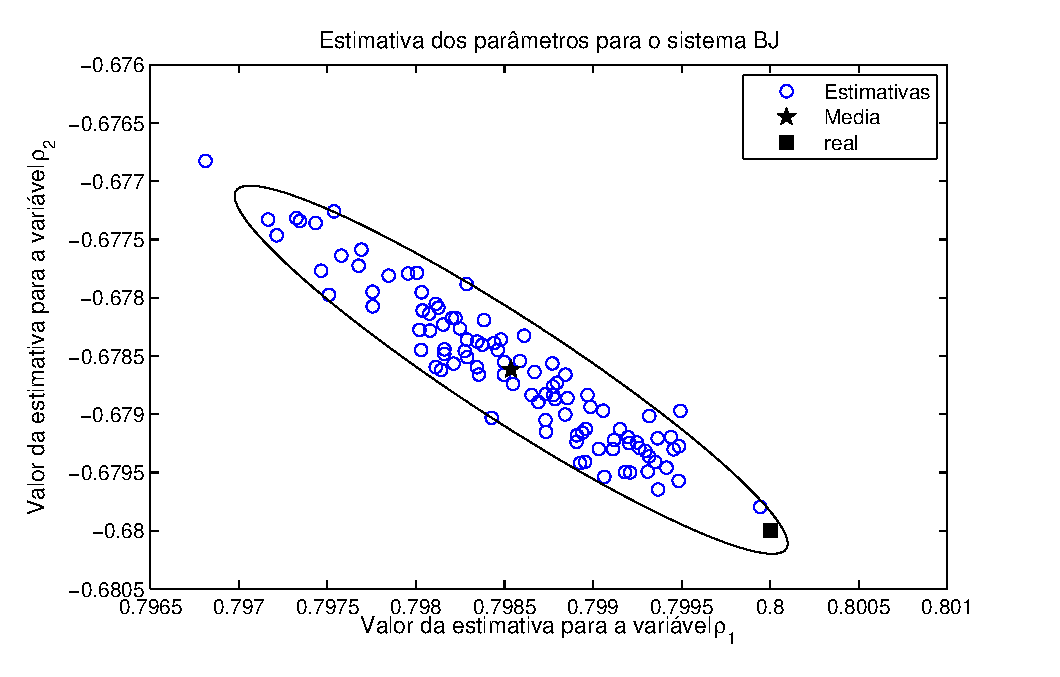
\includegraphics[width=0.95\columnwidth]{figures/vrft_bj_M10_var02.eps}
	\caption{100 estimativas Monte Carlo dos par�metros $\theta_1$ e $\theta_2$ para o controlador apresentado em
	\eqref{eq:vrft_methos_ex_bj_c} com um ru�do de vari�ncia de $\sigma_e^2=0.02$.}
	\label{fig:vrft_bj_M10_var02}
\end{figure}

\begin{figure}[htbp]
	\center
	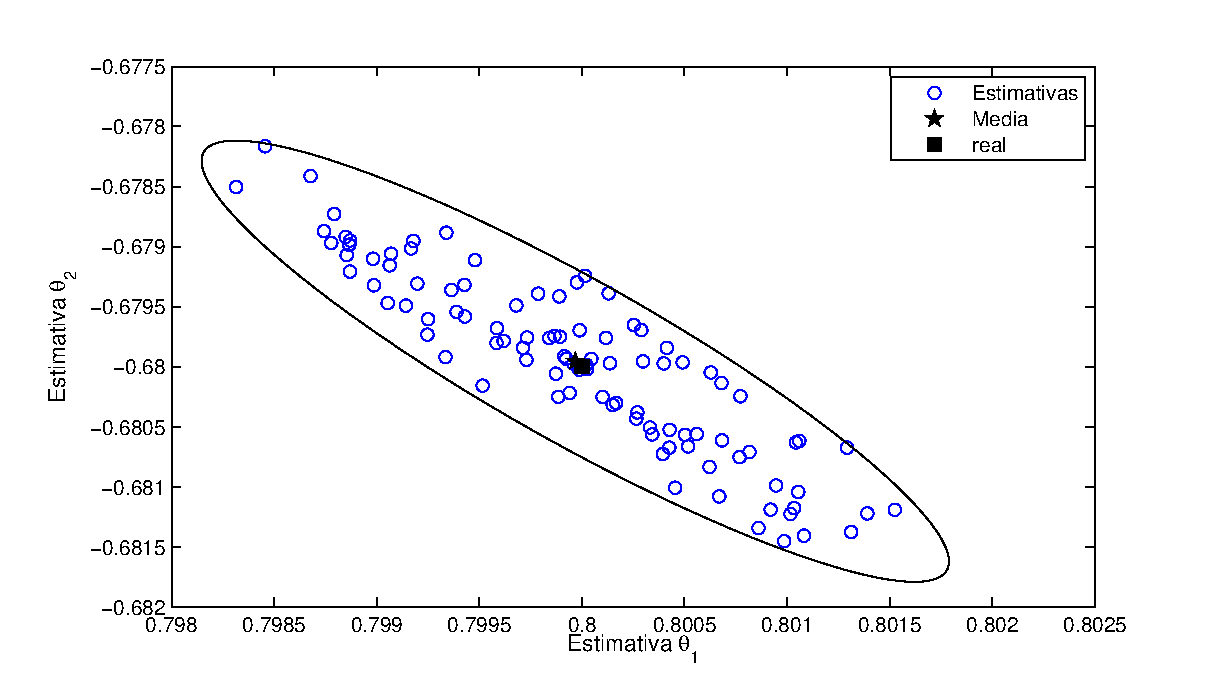
\includegraphics[width=0.95\columnwidth]{figures/vrft_bj_M10_var02_iv.eps}
	\caption{Resultado das 100 estimativas de Monte Carlo dos par�metros $\theta_1$ e $\theta_2$ para o
	controlador apresentado em \eqref{eq:vrft_methos_ex_bj_c} com vari�ncia do
	ru�do de 0.02. Utilizando vari�veis instrumentais para estimar os par�metros.}
	\label{fig:vrft_bj_M10_var02_iv}
\end{figure}

Observa-se que o erro de polariza��o foi minimizado e que o resultado obtido possui um custo $J_{VR}^N(\theta)
= 5.1242$ e a vari�ncia dos par�metros estimados foi de $0.5064\times10^{-6}$ para $\theta_1$ e de
$0.5495\times10^{-6}$ para $\theta_2$.

A fim de comparar o m�todo VRFT utilizando e n�o utilizando vari�veis instrumentais s�o apresentados abaixo as
Tabelas (\ref{table:vrft_method_bj}) e (\ref{table:vrft_method_bj_iv}) onde os custo $J_{y}$ e $J_{VR}^N$ s�o
apresentados para diferentes valores de vari�ncia do ru�do para o mesmo sistema BJ.

\begin{table*}[htbp]
\begin{center}
\caption{Valor dos custos $J_{VR}^N$ e $J_{y}$ al�m da vari�ncia das estimativas para diferentes valores de $\sigma_e^2$
quando o m�todo VRFT n�o utiliza vari�veis instrumentais para a estimativa dos par�metros $\theta$}
\label{table:vrft_method_bj}
\begin{tabular}{ccccc}
\hline
        Vari�ncia $\sigma_e^2$ & $J_{VR}^N(\theta)$ & $J_y(\theta)$ & M�dia $\theta_1$ & M�dia $\theta_2$  \\
\hline
	 0.1 	 & 	 4.87826e-02 	 & 	 2.15324e-02 	 & 	 0.76178 	 & 	 0.64466 \\ 
	 0.08 	 & 	 3.26789e-02 	 & 	 1.35688e-02 	 & 	 0.7759 	 & 	 0.65765 \\ 
	 0.06 	 & 	 1.80426e-02 	 & 	 7.86422e-03 	 & 	 0.78597 	 & 	 0.66715 \\ 
	 0.05 	 & 	 1.19341e-02 	 & 	 5.52796e-03 	 & 	 0.79017 	 & 	 0.67088 \\ 
	 0.04 	 & 	 7.54289e-03 	 & 	 3.65088e-03 	 & 	 0.79351 	 & 	 0.67396 \\ 
	 0.01 	 & 	 4.89481e-04 	 & 	 2.11052e-04 	 & 	 0.79962 	 & 	 0.67965 \\ 
	 0.008 	 & 	 3.25810e-04 	 & 	 1.83444e-04 	 & 	 0.79968 	 & 	 0.67969 \\ 
	 0.005 	 & 	 1.20816e-04 	 & 	 5.42193e-05 	 & 	 0.7999 	 & 	 0.67991 \\ 
	 0.003 	 & 	 4.73517e-05 	 & 	 2.28052e-05 	 & 	 0.79996 	 & 	 0.67996 \\ 
	 0.001 	 & 	 5.02347e-06 	 & 	 2.77267e-06 	 & 	 0.8 	     & 	 0.68 \\ 
\hline
\end{tabular}
\end{center}
\end{table*} 
   

\begin{table*}[htbp]
\begin{center}
\caption{Valor dos custos $J_{VR}^N$ e $J_{y}$ al�m da  vari�ncia das estimativas para diferentes valores de
$\sigma_e^2$ quando o m�todo VRFT utiliza vari�veis instrumentais para a estimativa dos par�metros $\theta$}
\label{table:vrft_method_bj_iv}
\begin{tabular}{ccccc}
\hline
        Vari�ncia $\sigma_e^2$ & $J_{VR}^N(\theta)$ & $J_{y}(\theta)$  & M�dia $\theta_1$ & M�dia $\theta_2$  \\
\hline
	 0.1 	 & 	 5.19132e-02 	 & 	 4.14964e-04 	 & 	 0.79936 	 & 	 0.67971 \\ 
	 0.08 	 & 	 3.31577e-02 	 & 	 2.96000e-04 	 & 	 0.80037 	 & 	 0.68007 \\ 
	 0.06 	 & 	 1.70932e-02 	 & 	 2.17256e-04 	 & 	 0.79989 	 & 	 0.67969 \\ 
	 0.05 	 & 	 1.27803e-02 	 & 	 3.14017e-05 	 & 	 0.80006 	 & 	 0.68005 \\ 
	 0.04 	 & 	 7.72145e-03 	 & 	 9.43578e-05 	 & 	 0.79996 	 & 	 0.68006 \\ 
	 0.01 	 & 	 5.00316e-04 	 & 	 3.20694e-05 	 & 	 0.80005 	 & 	 0.68003 \\ 
	 0.008 	 & 	 3.44326e-04 	 & 	 2.93508e-05 	 & 	 0.80001 	 & 	 0.68004 \\ 
	 0.005 	 & 	 1.19855e-04 	 & 	 6.96916e-06 	 & 	 0.79999 	 & 	 0.68 \\ 
	 0.003 	 & 	 4.22380e-05 	 & 	 6.33696e-06 	 & 	 0.80001 	 & 	 0.68001 \\ 
	 0.001 	 & 	 5.08709e-06 	 & 	 1.18016e-06 	 & 	 0.8 	 	 & 	 0.68 \\ 
\hline
\end{tabular}
\end{center}
\end{table*}

Utilizando vari�veis instrumentais observa-se que o custo $J_{y}(\theta)$ � significativamente mais baixo
quando comparado com o m�todo onde n�o s�o utilizadas vari�veis instrumentais, corroborando com o que foi apresentado na
se��o (\ref{sec:dbcd_vrft_framework_noise}).

%===============================================================================
\subsubsection{Controlador PID - sistema ARX}
\label{sec:dbcd_vrft_examples_pid_arx}
%===============================================================================

Considere o sistema real definido pefinido pelo modelo ARX:

\begin{equation}
G_{ 0 }(z)=\frac { z }{ (z-0.9)(z-0.8) } ,\quad \quad \quad H_{ 0 }(z)=\frac { z^2 }{ (z-0.9)(z-0.8) } 
\nonumber
\end{equation}

Deseja-se que o sistema em malha fechada comporte-se como:

\begin{equation}
T_d(z)=\frac { 0.4 }{ z-0.6 }
\label{eq:vrft_methos_ex_arx_M}
\end{equation}

Tem-se assim que o controlador ideal � definido por:

\begin{equation}
C_d(z)=\frac{T_d(z)}{G_0(z)(1-T_d(z))}=\frac { 0.4(z - 0.9)(z-0.8) }{ z(z-1) }
\label{eq:vrft_methos_ex_arx_cd}
\end{equation}

Observa-se que este controlador pode ser representado como um controlador
{\it{PID}} como em: 

\begin{equation}
C(z,\theta )=\frac { \theta _{ 1 }z^2+\theta _{ 2 }z+\theta _{ 3 } }{ z(z-1) } 
\label{eq:vrft_methos_ex_arx_c}
\end{equation}

Na Figura (\ref{fig:vrft_arx_M10_var005}) � apresentado o resultado da estimativa dos par�metros do
controlador quando n�o s�o utilizados vari�veis instrumentais. Juntamente com os valores das estimativas, � apresentado
o elips�ide de $\xi^2=95\%$ de confian�a. Obteve-se desta forma um custo $J_{VR}^N(\theta) = 2.5008\times10^{-5}$ e
$J_{y}(\theta) = 1.7746\times10^{-5}$ al�m de uma vari�ncia para as estimativas de $1.0\times10^{-7} \; [0.0364\;
0.1261\; 0.0377]$ para $\theta_1$, $\theta_2$ e $\theta_3$ respectivamente.

\begin{figure}[htbp] 
	\center 
	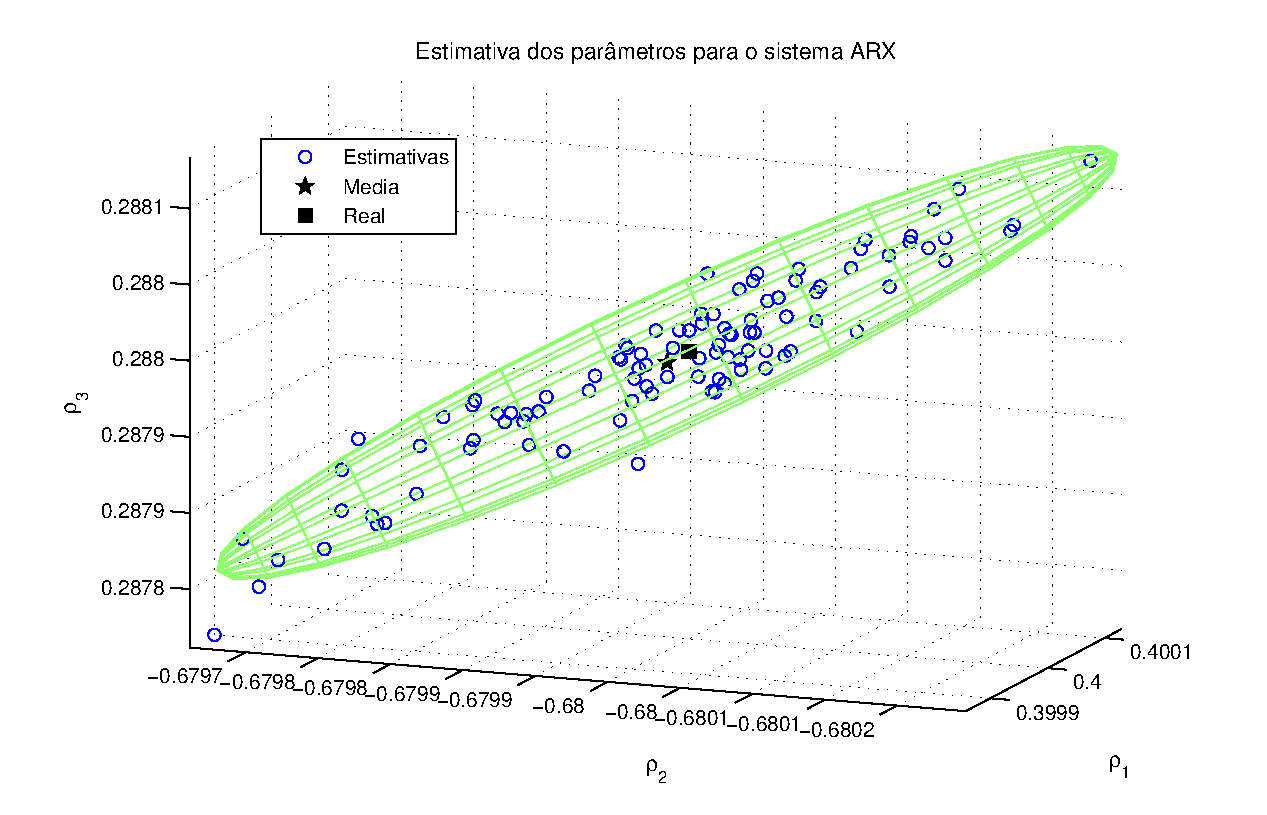
\includegraphics[width=0.95\columnwidth]{figures/vrft_arx_M10_var005_.eps}
	\caption{100 estimativas Monte Carlo dos par�metros $\theta_1$, $\theta_2$ e $\theta_3$ para o controlador
	apresentado em \eqref{eq:vrft_methos_ex_arx_c} com vari�ncia do ru�do $\sigma_e ^2=0.005$}
	\label{fig:vrft_arx_M10_var005}
\end{figure}

Como j� foi observado a utiliza��o de vari�veis instrumentais melhora significativamente o erro de polariza��o existente
nas estimativas do m�todo VRFT quaando h� presen�a de ru�do. Desta forma as informa��es apresentadas a seguir ser�o
feitas utilizando vari�veis instrumentais. Na figura (\ref{fig:vrft_arx_M10_var05_iv}) � apresentado a estimativa dos
par�metros do controlador para um ru�do de vari�ncia $\sigma_e ^2=0.05$. Observa-se que n�o h� erro de polariza��o nas
estimativas. O custo para esta, e outas, estimativas � apresentado na Tabela (\ref{table:vrft_method_arx_iv}).

\begin{figure}[htbp] 
	\center 
	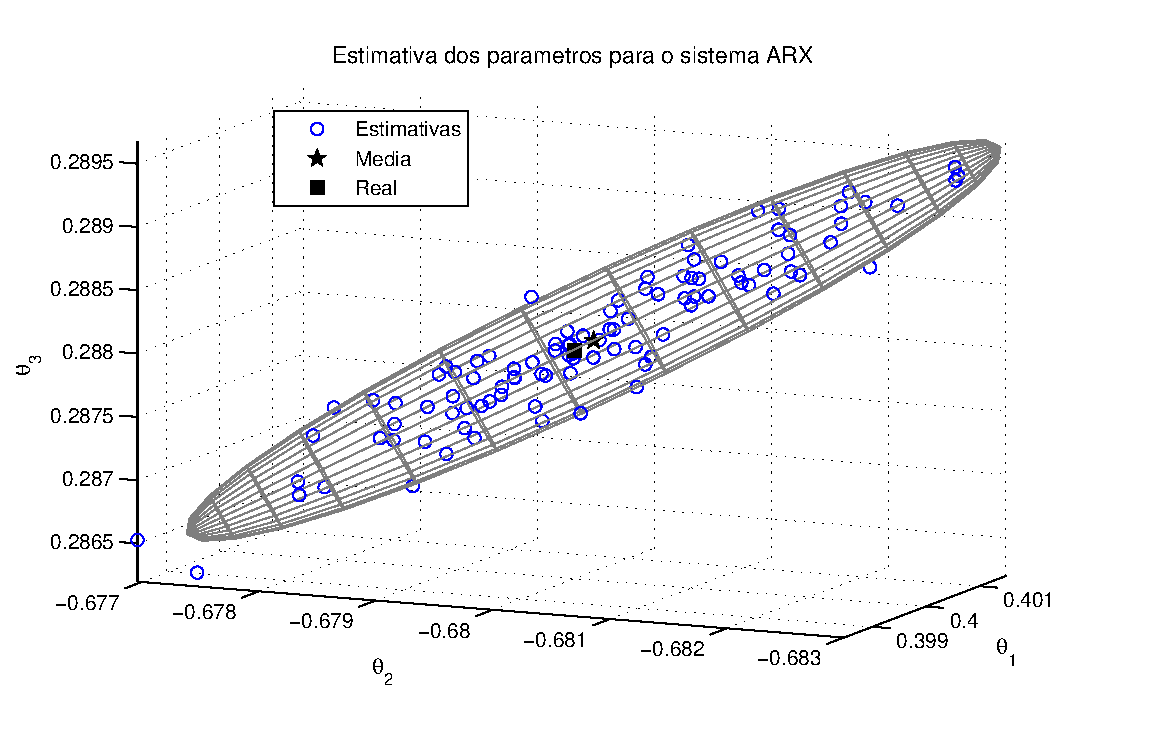
\includegraphics[width=0.95\columnwidth]{figures/vrft_arx_M10_var05_iv.eps}
	\caption{100 estimativas Monte Carlo dos par�metros $\theta_1$, $\theta_2$ e $\theta_3$ para o controlador
	apresentado em \eqref{eq:vrft_methos_ex_arx_c} com vari�ncia do ru�do $\sigma_e ^2=0.05$ utilizando
	vari�veis instrumentais}
	\label{fig:vrft_arx_M10_var05_iv}
\end{figure}


\begin{table*}[htbp]
\begin{center}
\caption{Valor dos custos $J_{VR}^N$ e $J_{y}$ al�m da  vari�ncia das
estimativas para diferentes valores de $\sigma_e^2$ quando o m�todo
VRFT utiliza vari�veis instrumentais para a estimativa dos par�metros $\theta$ do controlador
\eqref{eq:vrft_methos_ex_arx_c}}
\label{table:vrft_method_arx_iv}
\begin{tabular}{cccc}
\hline
        Vari�ncia $\sigma_e^2$ & $J_{VR}^N(\theta)$ &
        $J_{y}(\theta)$ & Vari�ncia estimativas $\theta$   \\
\hline
   0.1     & $10.0743\times10^{-3}$ &  2.2871$\times10^{-3}$ & $1\times10^{-5}\;[0.1253 \; 0.4683 \; 0.1600]$ \\
   0.06    & $ 3.6093\times10^{-3}$ &  1.1279$\times10^{-3}$ & $1\times10^{-5}\;[0.0516 \; 0.1793 \; 0.0575]$ \\
   0.05    & $ 2.5419\times10^{-3}$ &  1.2453$\times10^{-3}$ & $1\times10^{-5}\;[0.0344 \; 0.1237 \; 0.0416]$ \\
   0.04    & $ 1.6013\times10^{-3}$ &  0.5106$\times10^{-3}$ & $1\times10^{-6}\;[0.2195 \; 0.7908 \; 0.2379]$ \\
   0.01    & $10.0077\times10^{-5}$ & 13.7142$\times10^{-5}$ & $1\times10^{-7}\;[0.1552 \; 0.5469 \; 0.1822]$ \\
   0.005   & $ 2.5081\times10^{-5}$ & 10.3482$\times10^{-5}$ & $1\times10^{-7}\;[0.0406 \; 0.1260 \; 0.0375]$ \\
	0.001  & $ 0.1009\times10^{-5}$ &  2.0487$\times10^{-5}$ & $1\times10^{-9}\;[0.1277 \; 0.4035 \;0.1239]$	 \\
\hline
\end{tabular}
\end{center}
\end{table*}

%===============================================================================
\subsubsection{Controlador n�o pertence a classe}
\label{sec:dbcd_vrft_examples_not_in_class}
%===============================================================================

At� este ponto foram apresentados exemplos de uso do m�todo VRFT quando o controlador que leva o sistema para
o comportamento desejado $T_d(z)$ faz parte da classe escolhida para a identifica��o. Nesta se��o ser� apresentado um
exemplo onde a classe de modelos do controlador escolhida n�o consegue represetar o controlador ideal $C_d(z)$.

Considerando o sistema real descrito por:

\begin{equation}
G_{ 0 }(z)=\frac { 0.2(z-0.7) }{ (z-0.9)(z-0.5) } ,\quad \quad \quad H_{ 0 }(z)=\frac { z }{ z-0.3 } 
\nonumber
\end{equation}

Deseja-se que em malha fechada ele se comporte como em: 

\begin{equation}
T_d(z)=\frac { 0.16z }{ (z-0.6)^2 }
\label{eq:vrft_methos_ex_pid_not_M}
\end{equation}

Neste caso o controlador ideal � definido por

\begin{equation}
C_{ d }(z)=\frac { 0.8z(z-0.9)(z-0.5) }{ (z-1)(z-0.36)(z-0.7) } 
\label{eq:vrft_methos_ex_pid_not_cd}
\end{equation}

Para esta identifica��o optou-se por um controlador do tipo PID como em:
 
\begin{equation}
C(z,\theta )=\frac { \theta _{ 1 }z^2+\theta _{ 2 }z+\theta _{ 3 } }{ z(z-1) } 
\label{eq:vrft_methos_ex_pid_not_c}
\end{equation}

Observa-se que \eqref{eq:vrft_methos_ex_pid_not_c} n�o consegue representar todas as din�micas apresentadas em
\eqref{eq:vrft_methos_ex_pid_not_cd}. Utilizando o procedimento descrito na Se��o
(\ref{sec:dbcd_vrft_framework_noise}) e o procedimento de experimento repetido, foram feitos 100 experimentos de
Monte Carlo e o resultado obtido para a m�dia das estimativas foi:

\begin{equation}
\theta_L =\left[ 0.8101 \quad -0.1691  \quad -0.3358 \right]
\nonumber
\end{equation}

onde o �ndice $L$ indica que este resultado foi obtido utilizando-se o filtro $L$.

Repetindo a simula��o, mas agora sem que o procedimento da utiliza��o do filtro $L$ descrito na se��o
(\ref{sec:dbcd_vrft_framework_noise}), obteve-se o resultado seguinte:

\begin{equation}
\theta =\left[ 0.5846 \quad -0.2108  \quad -0.1525 \right]
\nonumber
\end{equation}

Aplicando-se estes resultados ao controlador apresentado em \eqref{eq:vrft_methos_ex_pid_not_c} e de posse do
comportamento desejado para o sistema em malha fechada ($T_d(z)$) � poss�vel fazer um comparativo da resposta
ao salto unit�rio para o sistema utilizando os dois controladores obtidos. O resultado � apresentado na Figura
(\ref{fig:vrft_notinclass_step}).

\begin{figure}[htbp] 
	\center 
	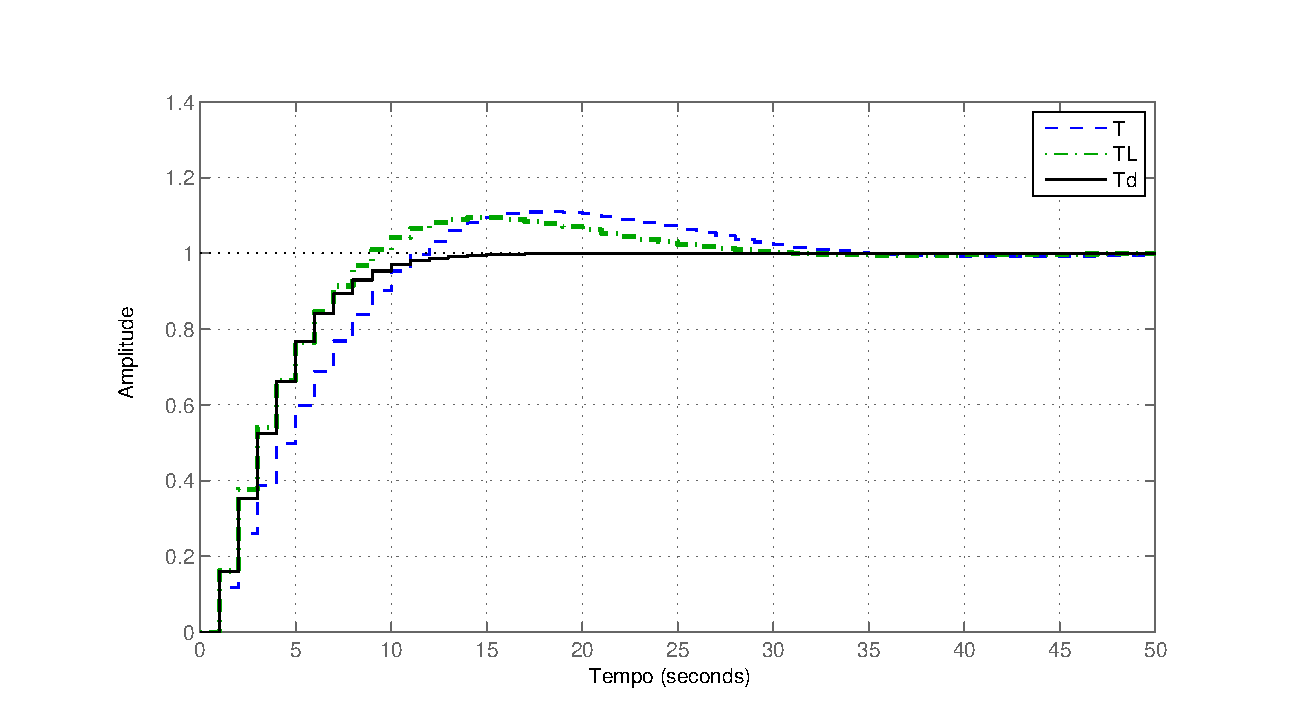
\includegraphics[width=0.85\columnwidth]{figures/vrft_notinclass_step.eps}
	\caption{Comparativo da resposta do sistema a um degrau unit�rio quando o controlador inserido � obtido pelo
	m�todo VRFT utilizando o filtro L e quando n�o se utiliza este artificio. O sistema foi simulado com um
	ru�do de vari�ncia $\sigma_e ^2=0.1$}
	\label{fig:vrft_notinclass_step}
\end{figure}

Observa-se que para o sistema que utiliza o controlador estimado utilizando-se o filtro $L$, a resposta ao
degrau unit�rio tem significativamente menos erro que o sistema utilizando o outro controlador. Ficando este
primeiro muito mais pr�ximo da fun��o $T_d(z)$ desejada.

Os custos destes dois sistemas � apresentado na Tabela (\ref{table:vrft_method_notinclass}).

\begin{table*}[htbp]
\begin{center}
\caption{Valor dos custos $J_{VR}^N$ e $J_{y}$ para o sistema controlado por $C(z)$ e $C_L(z)$}
\label{table:vrft_method_notinclass}
\begin{tabular}{ccc}
\hline
        Controlador & $J_{VR}^N(\theta)$ & $J_{y}(\theta)$ \\
\hline
	$C(z)$   & 0.2877 &  0.1270 \\
	$C_L(z)$ & 0.4481 &  0.0542 \\
\hline
\end{tabular}
\end{center}
\end{table*}

A fim de comparar as duas estimativas, na figura (\ref{fig:vrft_notinclass_bode}) � apresentado o diagrama de
Bode dos controladores obtidos (utilizando a m�dia das estimativas obtidas).

\begin{figure}[htbp] 
	\center 
	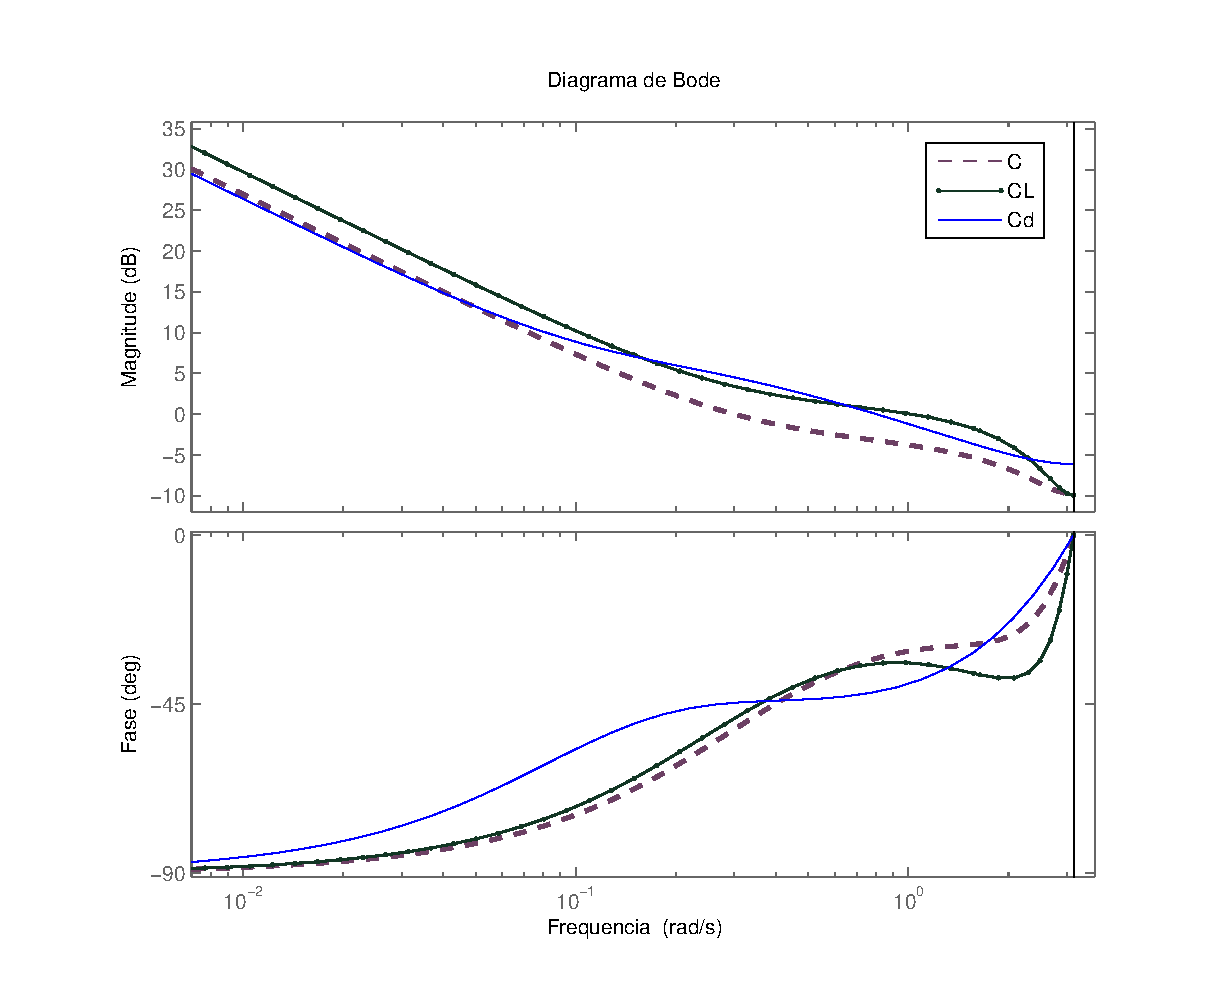
\includegraphics[width=0.85\columnwidth]{figures/vrft_notinclass_bode.eps}
	\caption{Diagrama de Bode para as fun��es de transfer�ncia dos controladores estimados utilizando VRFT com e
	sem o artificio do filtro L e vari�veis instrumentais}
	\label{fig:vrft_notinclass_bode}
\end{figure}


%===============================================================================
\section{Considera��es Finais}
\label{sec:vrft_conclusions}
%===============================================================================


%===============================================================================

